
\section{Introducció}

El següent projecte presenta un estudi de la mecànica de vol darrere d'una reentrada d'un vehicle a l'atmosfera terrestre.

En el retorn de l'espai, l'atmosfera terrestre es comporta com un fluid dens, el qual a velocitats orbitals es transforma en un gran obstacle que cal creuar. És necessari impactar amb l'atmosfera amb un precís angle de reentrada i velocitat per assegurar un aterratge segur segons \cite{archivo2}. 

Existeixen dos tipus de vehicles en la reentrada planetària destacats per \cite{adams} a l'atmosfera terrestre. Segons el tipus en concret, es determina completament el disseny d'aquests vehicles tripulats o dels vehicles no tripulats per a la reintroducció hipersònica a l'atmosfera terrestre des de l’espai.
\begin{itemize}
    \item \textbf{Balístics} (vehicles de reentrada, càpsula Mercury, etc.).
    \item \textbf{Sustentadors} (vehicles de reentrada maniobrables, càpsules Gemini i Apollo, HL-10, ACTIU, PRIME, X24-A, X24-B, etc.)
\end{itemize}

\begin{figure}[h]
    \centering
    \begin{minipage}{.55\textwidth}
        \centering
        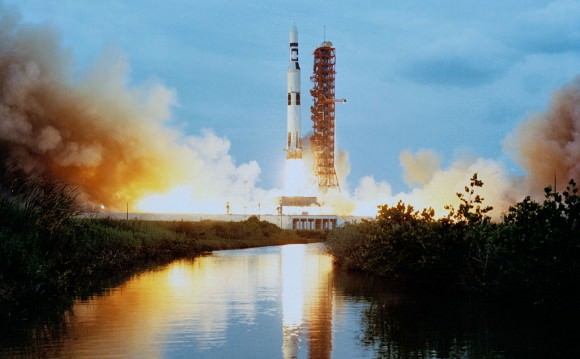
\includegraphics[height=5cm]{imagenes/00_general/saturnv.jpg}
        \captionof{figure}{Coet Saturn V. A partir de \cite{nasa_saturnv}}
    \end{minipage}%
    \begin{minipage}{.45\textwidth}
        \centering
        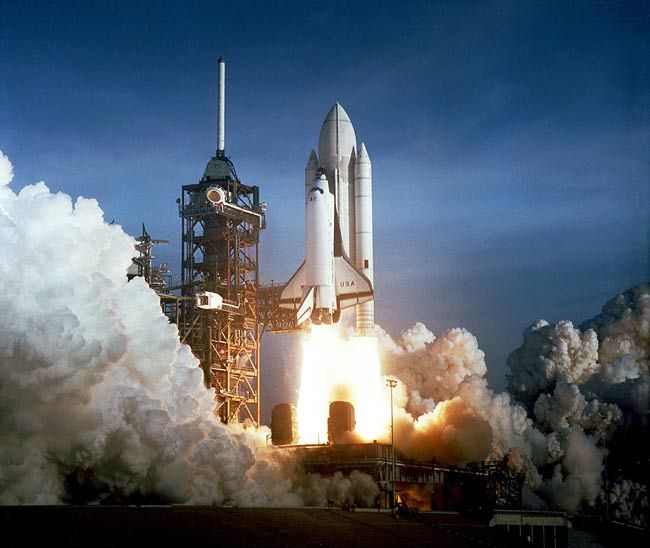
\includegraphics[height=5cm]{imagenes/00_general/spaceshuttle.jpg}
        \captionof{figure}{Space Shuttle. A partir de \cite{nasa_spaceshuttle}}
    \end{minipage}
\end{figure}





